\section{Tracking the Probe on a Deformable Surface}

\subsection{Mesh Following Algorithm}

After calibration, due to deformability and possible measurement errors, our rendered path in the virtual world will have segments that are above or below the virtual surface as shown in Figure \ref{pathsAboveAndBelow}. Because the path was recorded on the real surface, we want a visualization on the virtual surface of the probe's location on the real surface. We will thus do a transformation of the virtual path to better match where the real path traversed. Because we already calibrated the scale of the movements, the transformation will preserve arc length. Because the rotation was already calibrated, the orientation along the surface will be preserved.

\begin{figure}[ht]
\centering
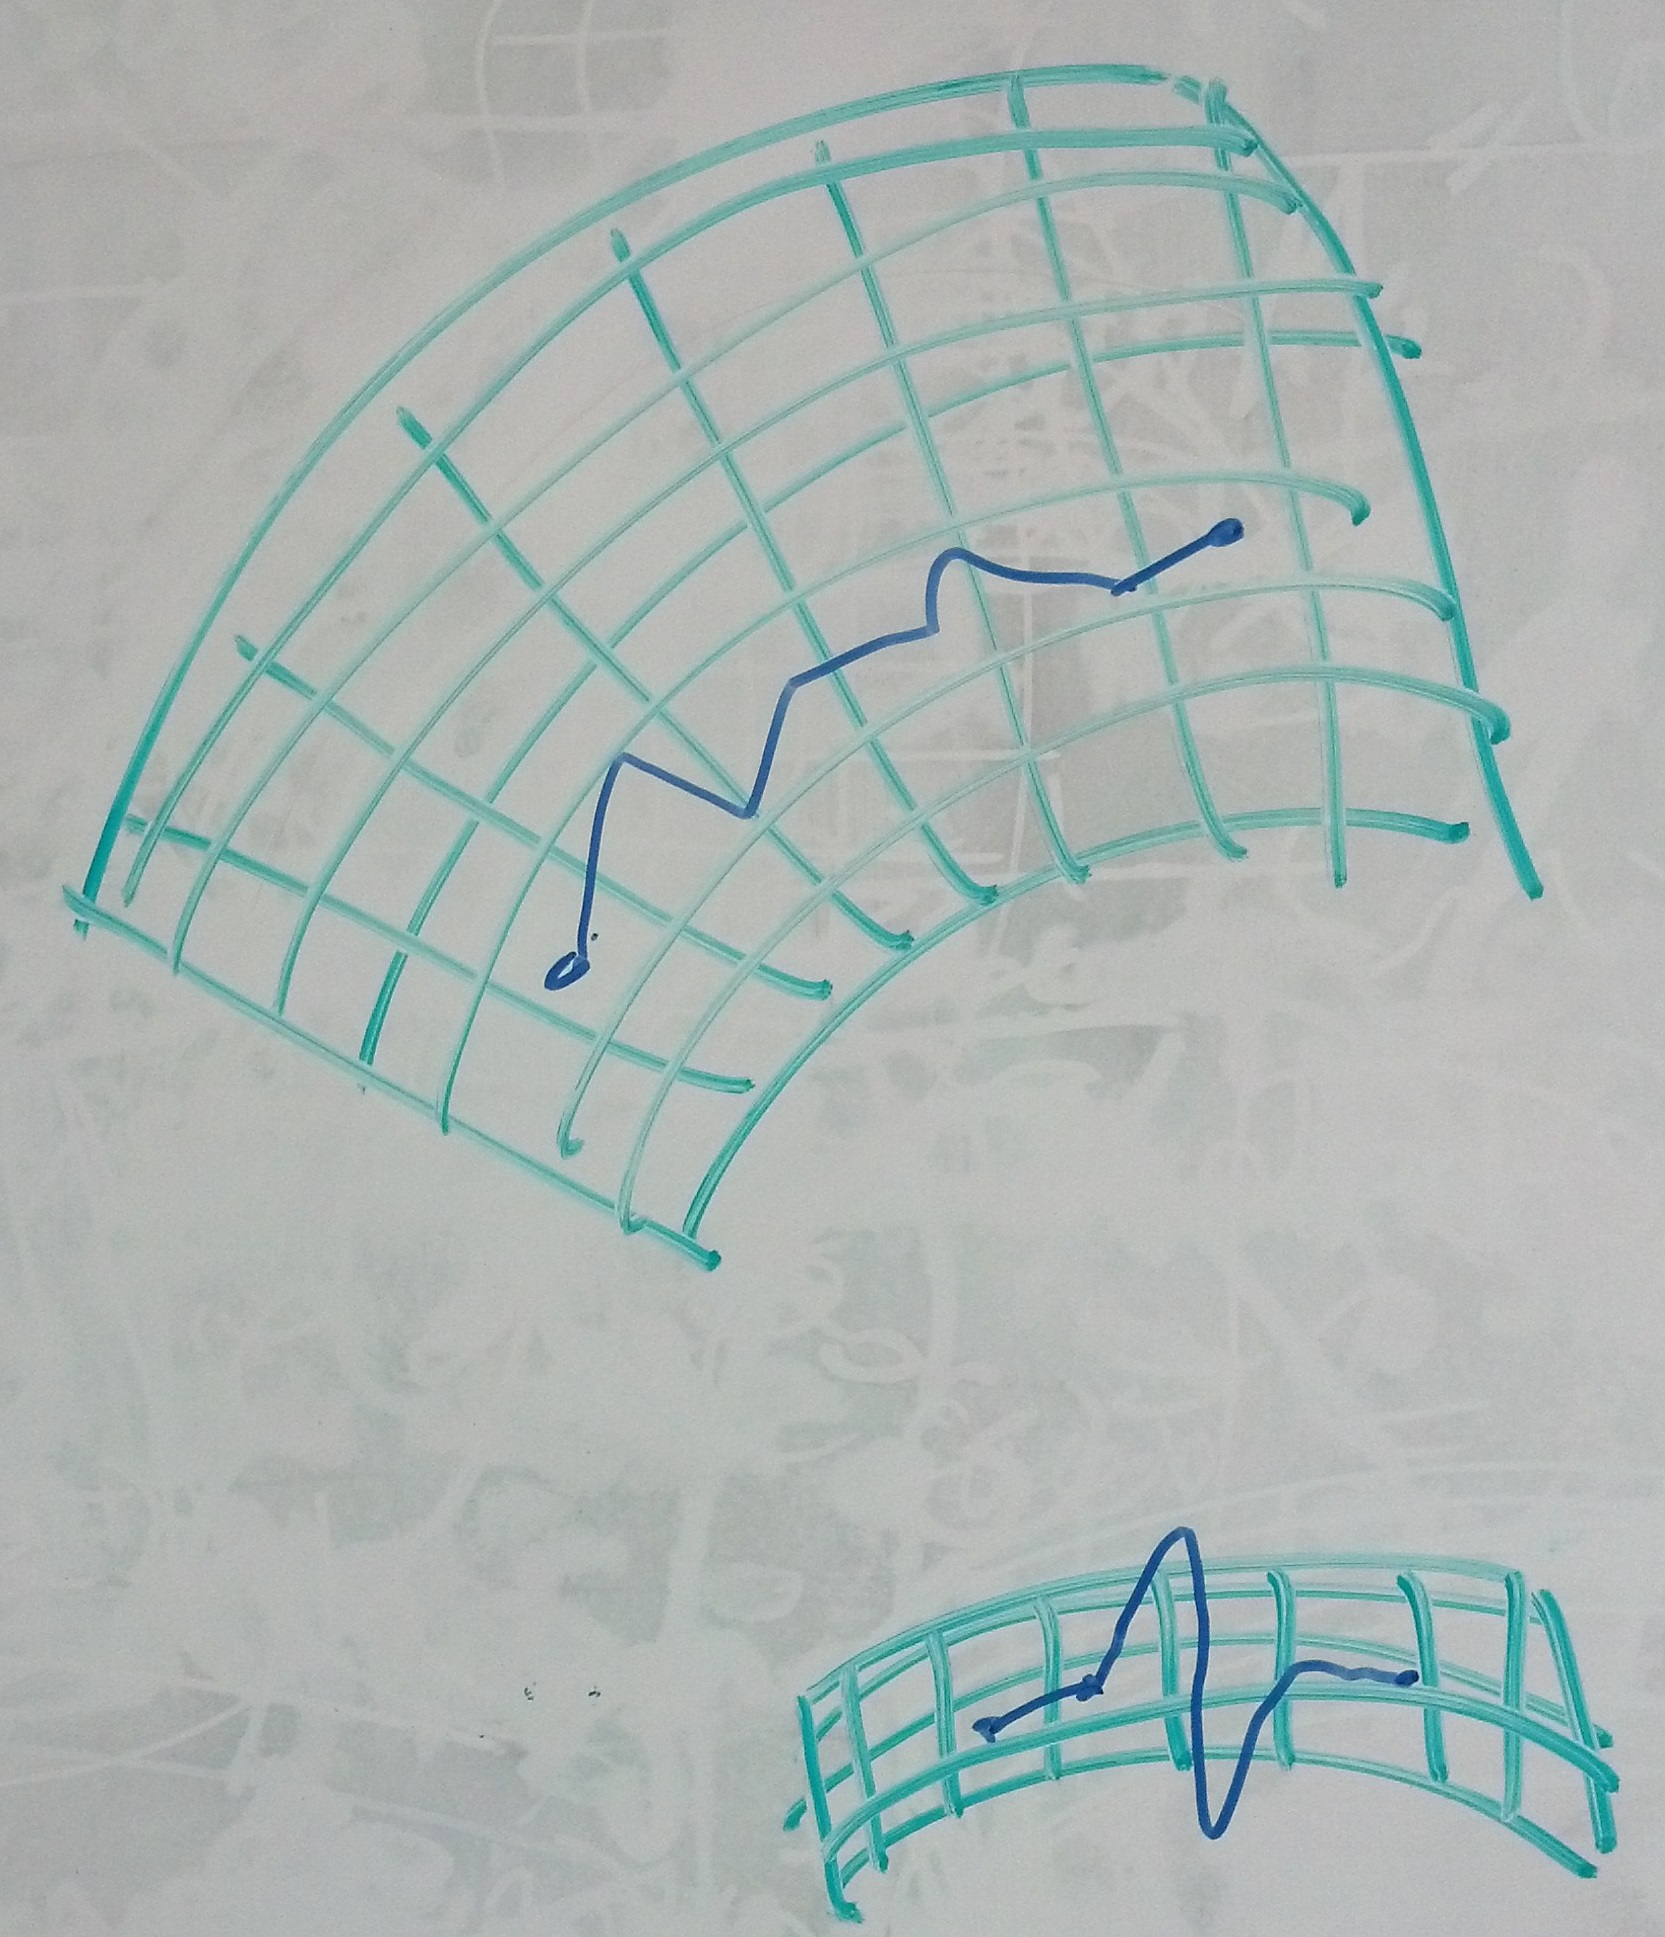
\includegraphics[width=\columnwidth]{pathaboveandbelow.jpg}
\caption{Path above and below surface}
\label{pathsAboveAndBelow}
\end{figure}

We have a known and rigid starting point $p_0$ on the triangular manifold mesh $M$ for our path (TODO: The fact that it is a triangular manifold mesh will be established in previous sections). The rest of the path is a set of $n$ segments $s_0,...,s_{n-1}$ where the starting point of $s_0$ is $p_0$ and the rest of the segments start at the point where the previous segment ended. We need a new set of segments that all lie on triangles of the mesh. Our goal is thus a new path consisting of $m$ points, $p_0, p_1,...,p_{m-1}$, such that each $p_i$ is on $M$ and for each $i>0$, $p_{i}$ and $p_{i-1}$ lie on the same triangle. \\
\\
After finding how the first segment follows the mesh, we will have a new start point on the mesh as well as $n-1$ segments that need to be projected onto the mesh. We can thus have an algorithm that finds a projection for a single vector and starting point and then recursively computes the rest of the path, below:.\\
\\
Project( $p$, $\{s_0,s_1,...,s_{n-1}\}$,$M$ ):\\
-Project $s_0$ onto $M$\\
-Get new start point $p'$\\
-Project( $p'$, $\{s_1,...,s_{n-1}\}$,$M$)\\ 
\\
When we project the first segment, we want it to follow the geodesic path along the mesh. **JUSTIFY THIS**. We will therefore flatten the mesh around the local area that the segment traverses. Our segments are short enough that if $\epsilon$ is the length, then the $\epsilon$-neighborhood around the start point will be homeomorphic to $R^2$ thus the flattening will exist. We will denote $T$ as the triangle where the starting point lies. We will develop a secondary mesh $M_0$ that consists of $T$ and its neighbors. The triangles in $M_0$ will be rotated so that they lie on the same plane as $T$. \\
\\
We will let $v$ be the vector for our input segment, $N$ be the normal of $T$, and $E$ be the resultant vector that is both on the plane formed by $N$ and $v$ and has an acute angle with $v$. Having a vector with both of those properties ensures that we are preserving orientation along the surface. As can be observed in figure \ref{vectordiagram}, the following equation will then hold
\[
E + proj_N(v) = v
\]

\begin{figure}[ht]
\centering
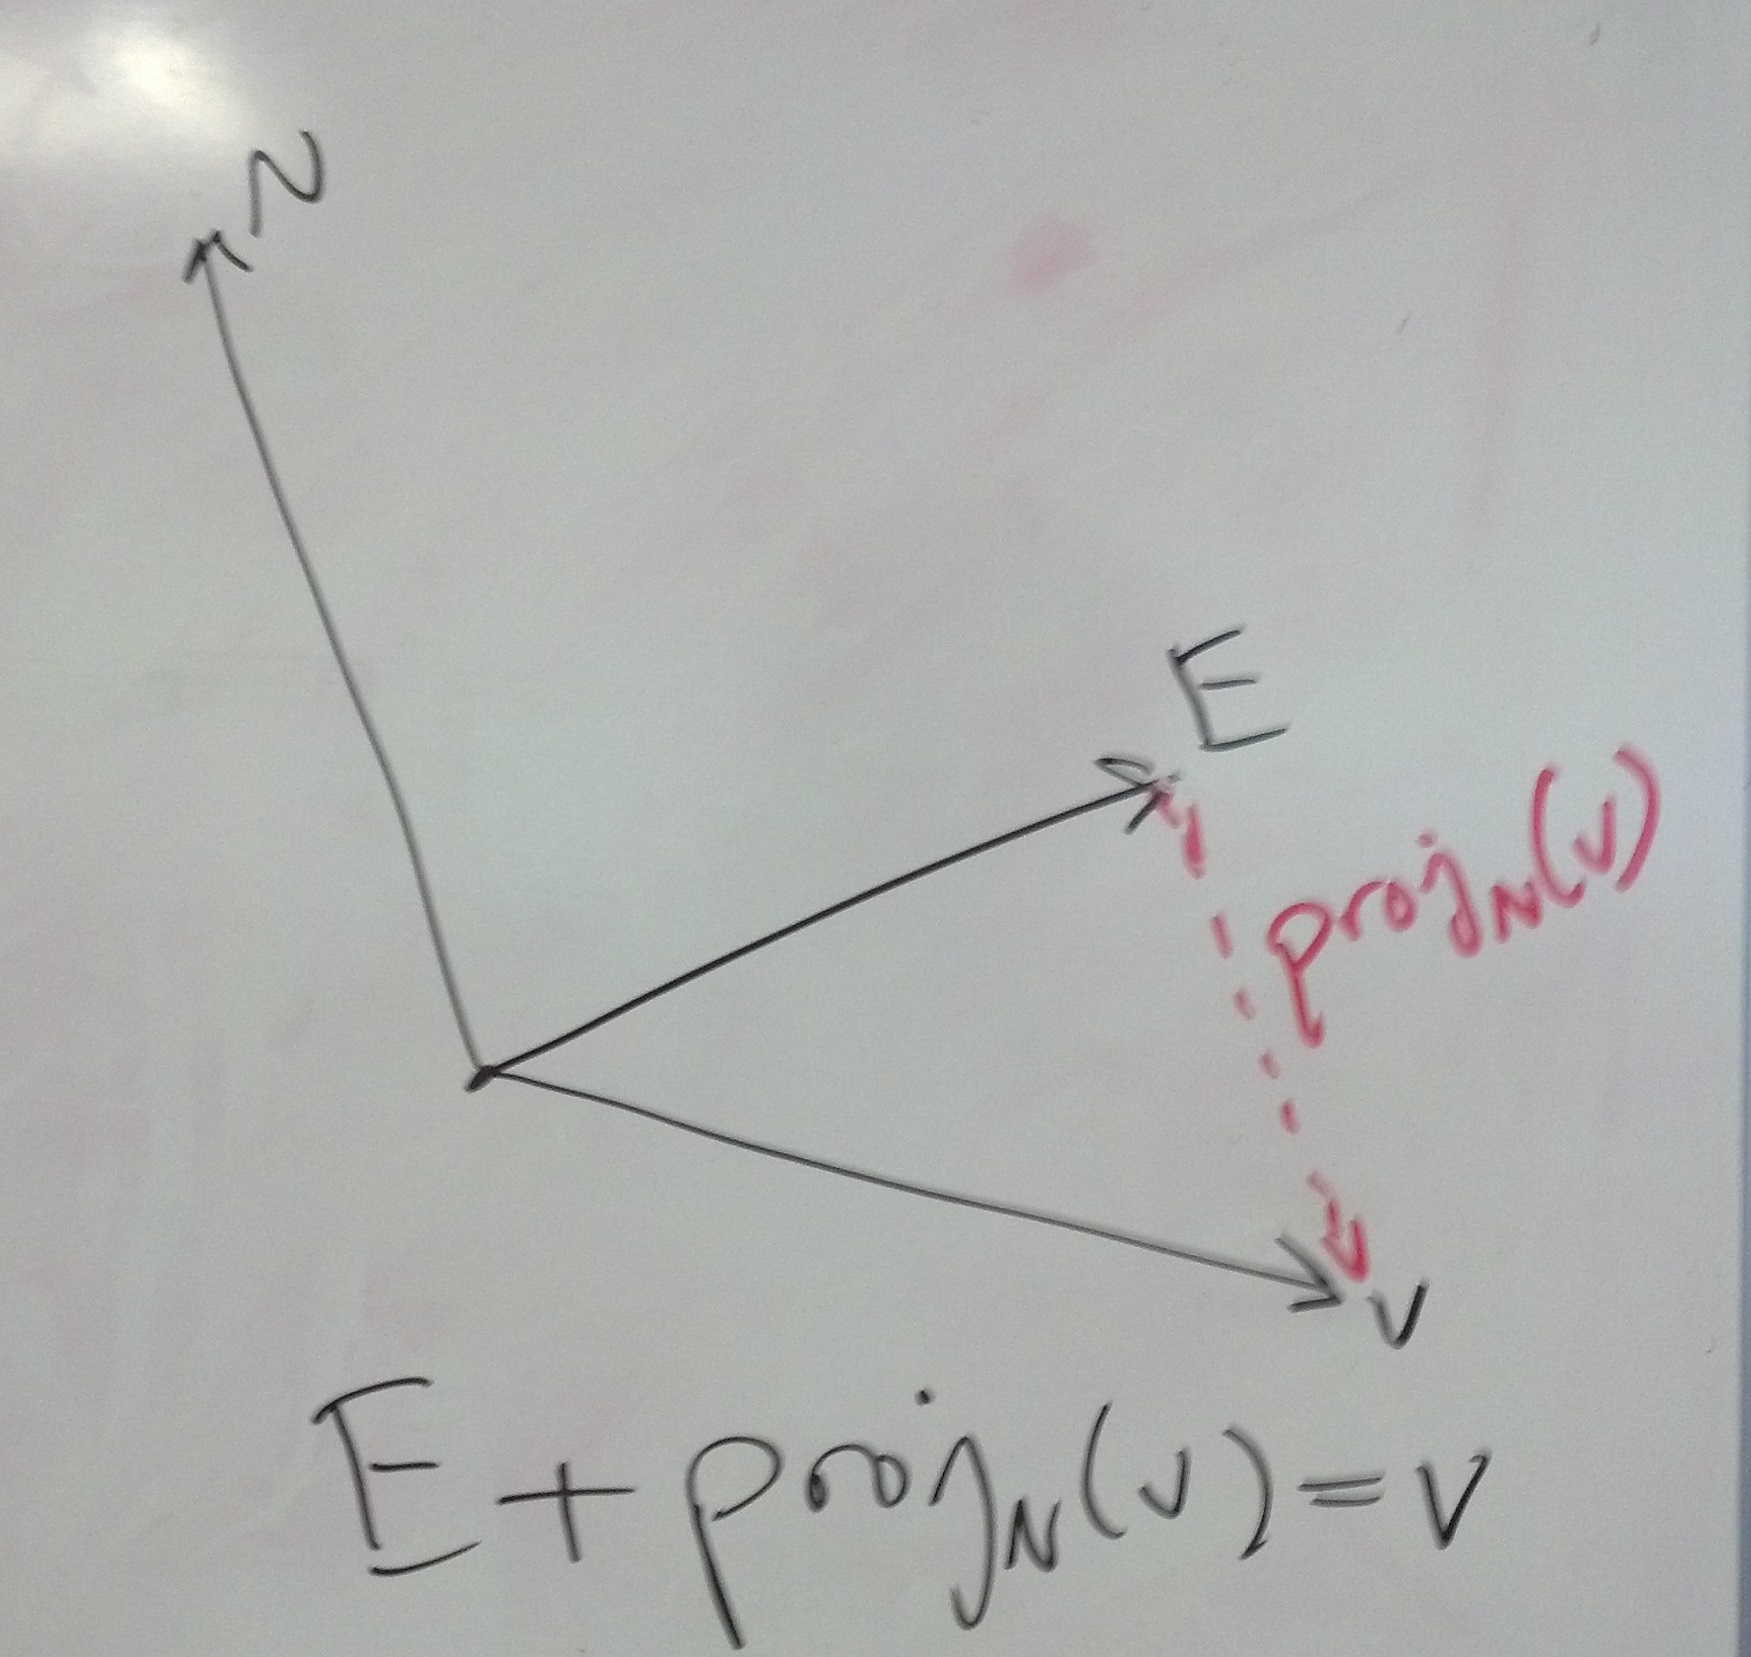
\includegraphics[width=\columnwidth]{vectordiagram.jpg}
\caption{The segment vector, normal, and projected vector}
\label{vectordiagram}
\end{figure}

Thus, the following equation will get us $E$
\[
E = v - proj_N(v)
\]
This can be further simplified to say
\[
E = v - N(v.N)
\]
We will draw $E$ on the mesh $M_0$. If the segment lies entirely inside $M_0$ as in Figure \ref{flatteningDiagram_oneTriangle}, then we are done. Otherwise, we will add triangles to $M_0$, rotate them to be on the same plane as $T$, and extend $E$ onto them, as in Figure \ref{flatteningDiagram_neighborhood}.By the manifold property, the flattening will always exists **JUSTIFY THIS** and this path will thus be a geodesic path **JUSTIFY THIS**. This will leave us with a series of connected points either on the interior or edges of each of the triangles. These points are computed in each triangle's coordinate system, so that the coordinates of these points in $M$ are easily computed and those coordinates are used to get the path that follows the mesh.\\
In the total, the algorithm takes in a starting point on the mesh $p$, a sequence of segments that starts from that point, and a triangular manifold mesh $M$. It outputs a sequence of points $\{ p_0, p_1, ... , p_m\}$ that lie on the mesh. The pseudo-code is in algorithm \ref{pseudocode}.\\
\\
\begin{algorithm}[t]
Input: Starting point $p_0$, Segments $s_0,...,s_m$, Mesh $M$\;
Set $p \leftarrow p_0$ \;
Initialize list $P$ of points and add $p_0$ to it \;
Set $T$ to be the triangle of $p_0$ \;
\For{each segment $s_i$ in order}{
	Set $N$ to be normal for $T$\;
	Clear $M_0$ and add $T$ to it \;
	Set $v$ to be the vector for $s_i$ \;
	Set $E \leftarrow v - N(v.N)$ \;
	Add Triangles to $M_0$ until $p+E$ is in $M_0$ \;
	Add points computed to $P$ \;
	Set $p$ $\leftarrow$ $p+E$ \;
}
\While{{\bf true}}{
		\While{top element of $E_M$ is positive}{
			Pop top element and move the data unit to its destination \;
			Update $E_M$ and $E_C$ \;
		}
		\eIf{there is more space for redundancy}{
		Pop top element and copy the data unit to its destination \;
		Update $E_M$ and $E_C$ \;
		}{{\bf break}}
}
\caption{Pseudo-code for our algorithm}
\label{pseudocode}
\end{algorithm}

\begin{figure}[ht]
\centering
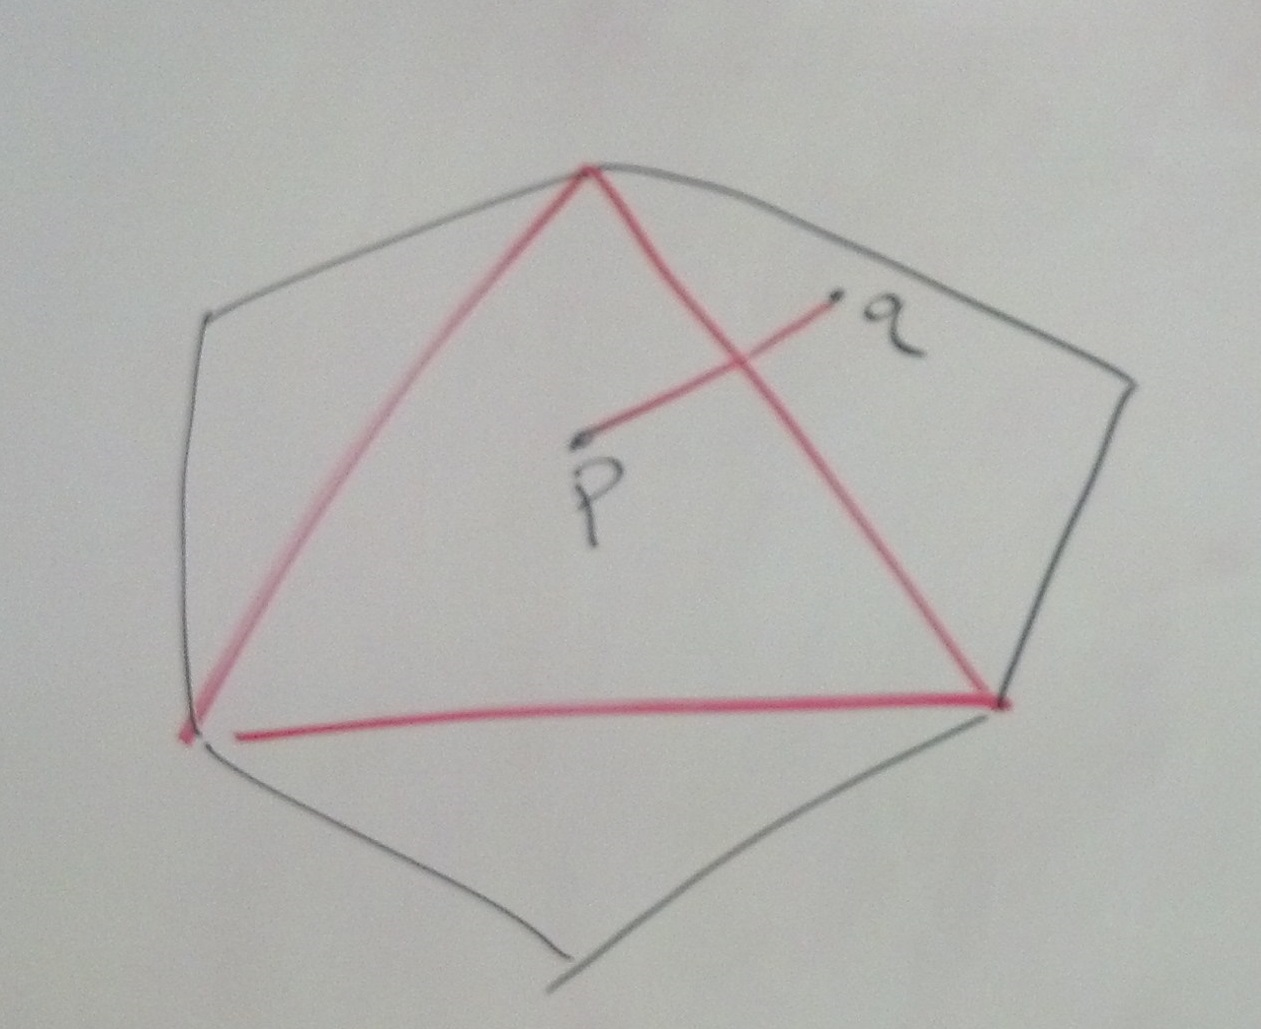
\includegraphics[width=\columnwidth]{flatteningdiagram_oneTriangleAndNeighbors.jpg}
\caption{The triangle at $p$ and its neighbors}
\label{flatteningDiagram_oneTriangle}
\end{figure}
\begin{figure}[ht]
\centering
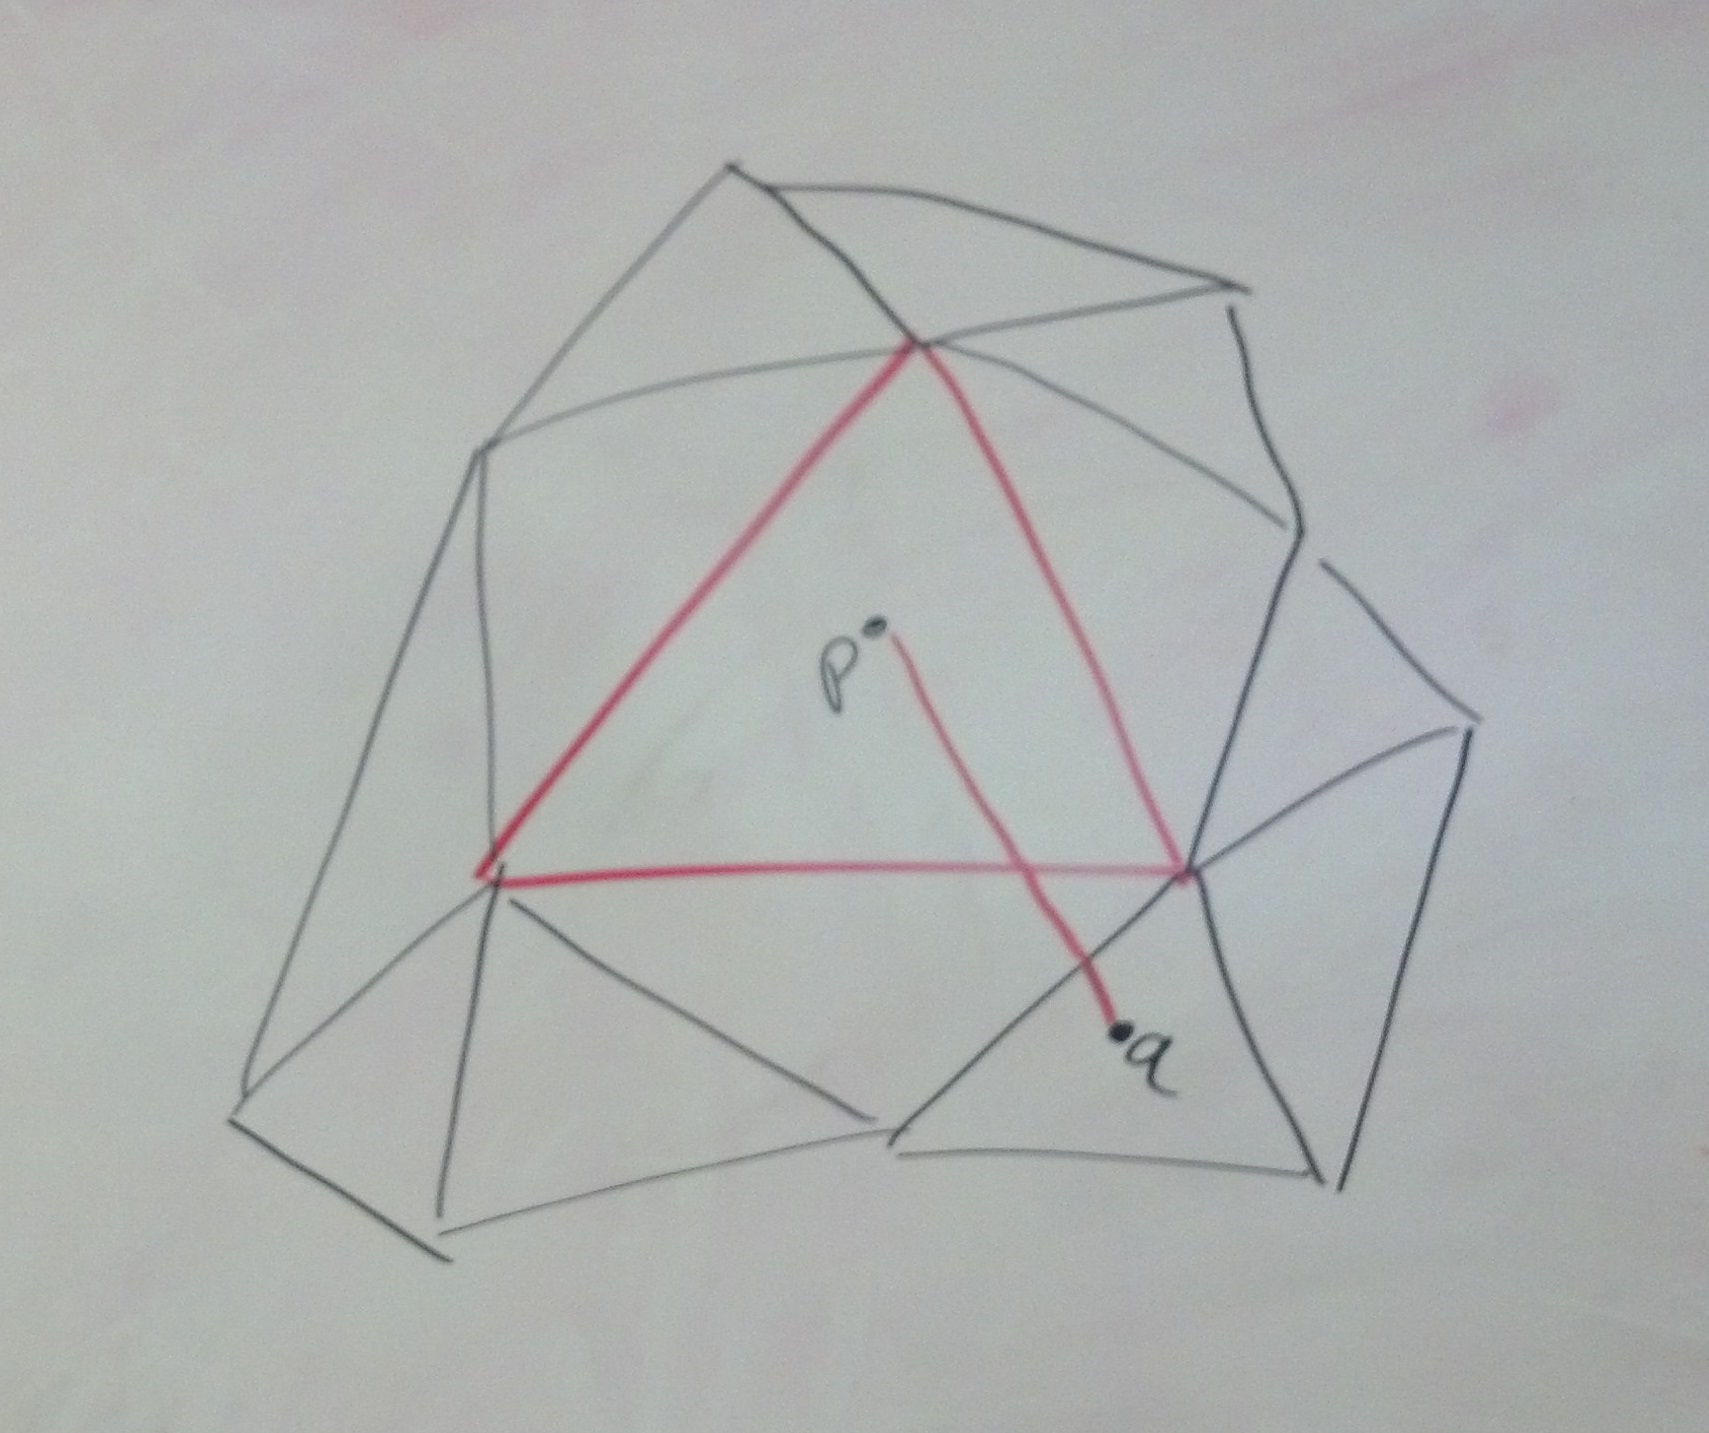
\includegraphics[width=\columnwidth]{flatteningdiagram_neighborhood.jpg}
\caption{The triangles in the neighborhood around $p$}
\label{flatteningDiagram_neighborhood}
\end{figure}

\begin{figure}[ht]
\centering
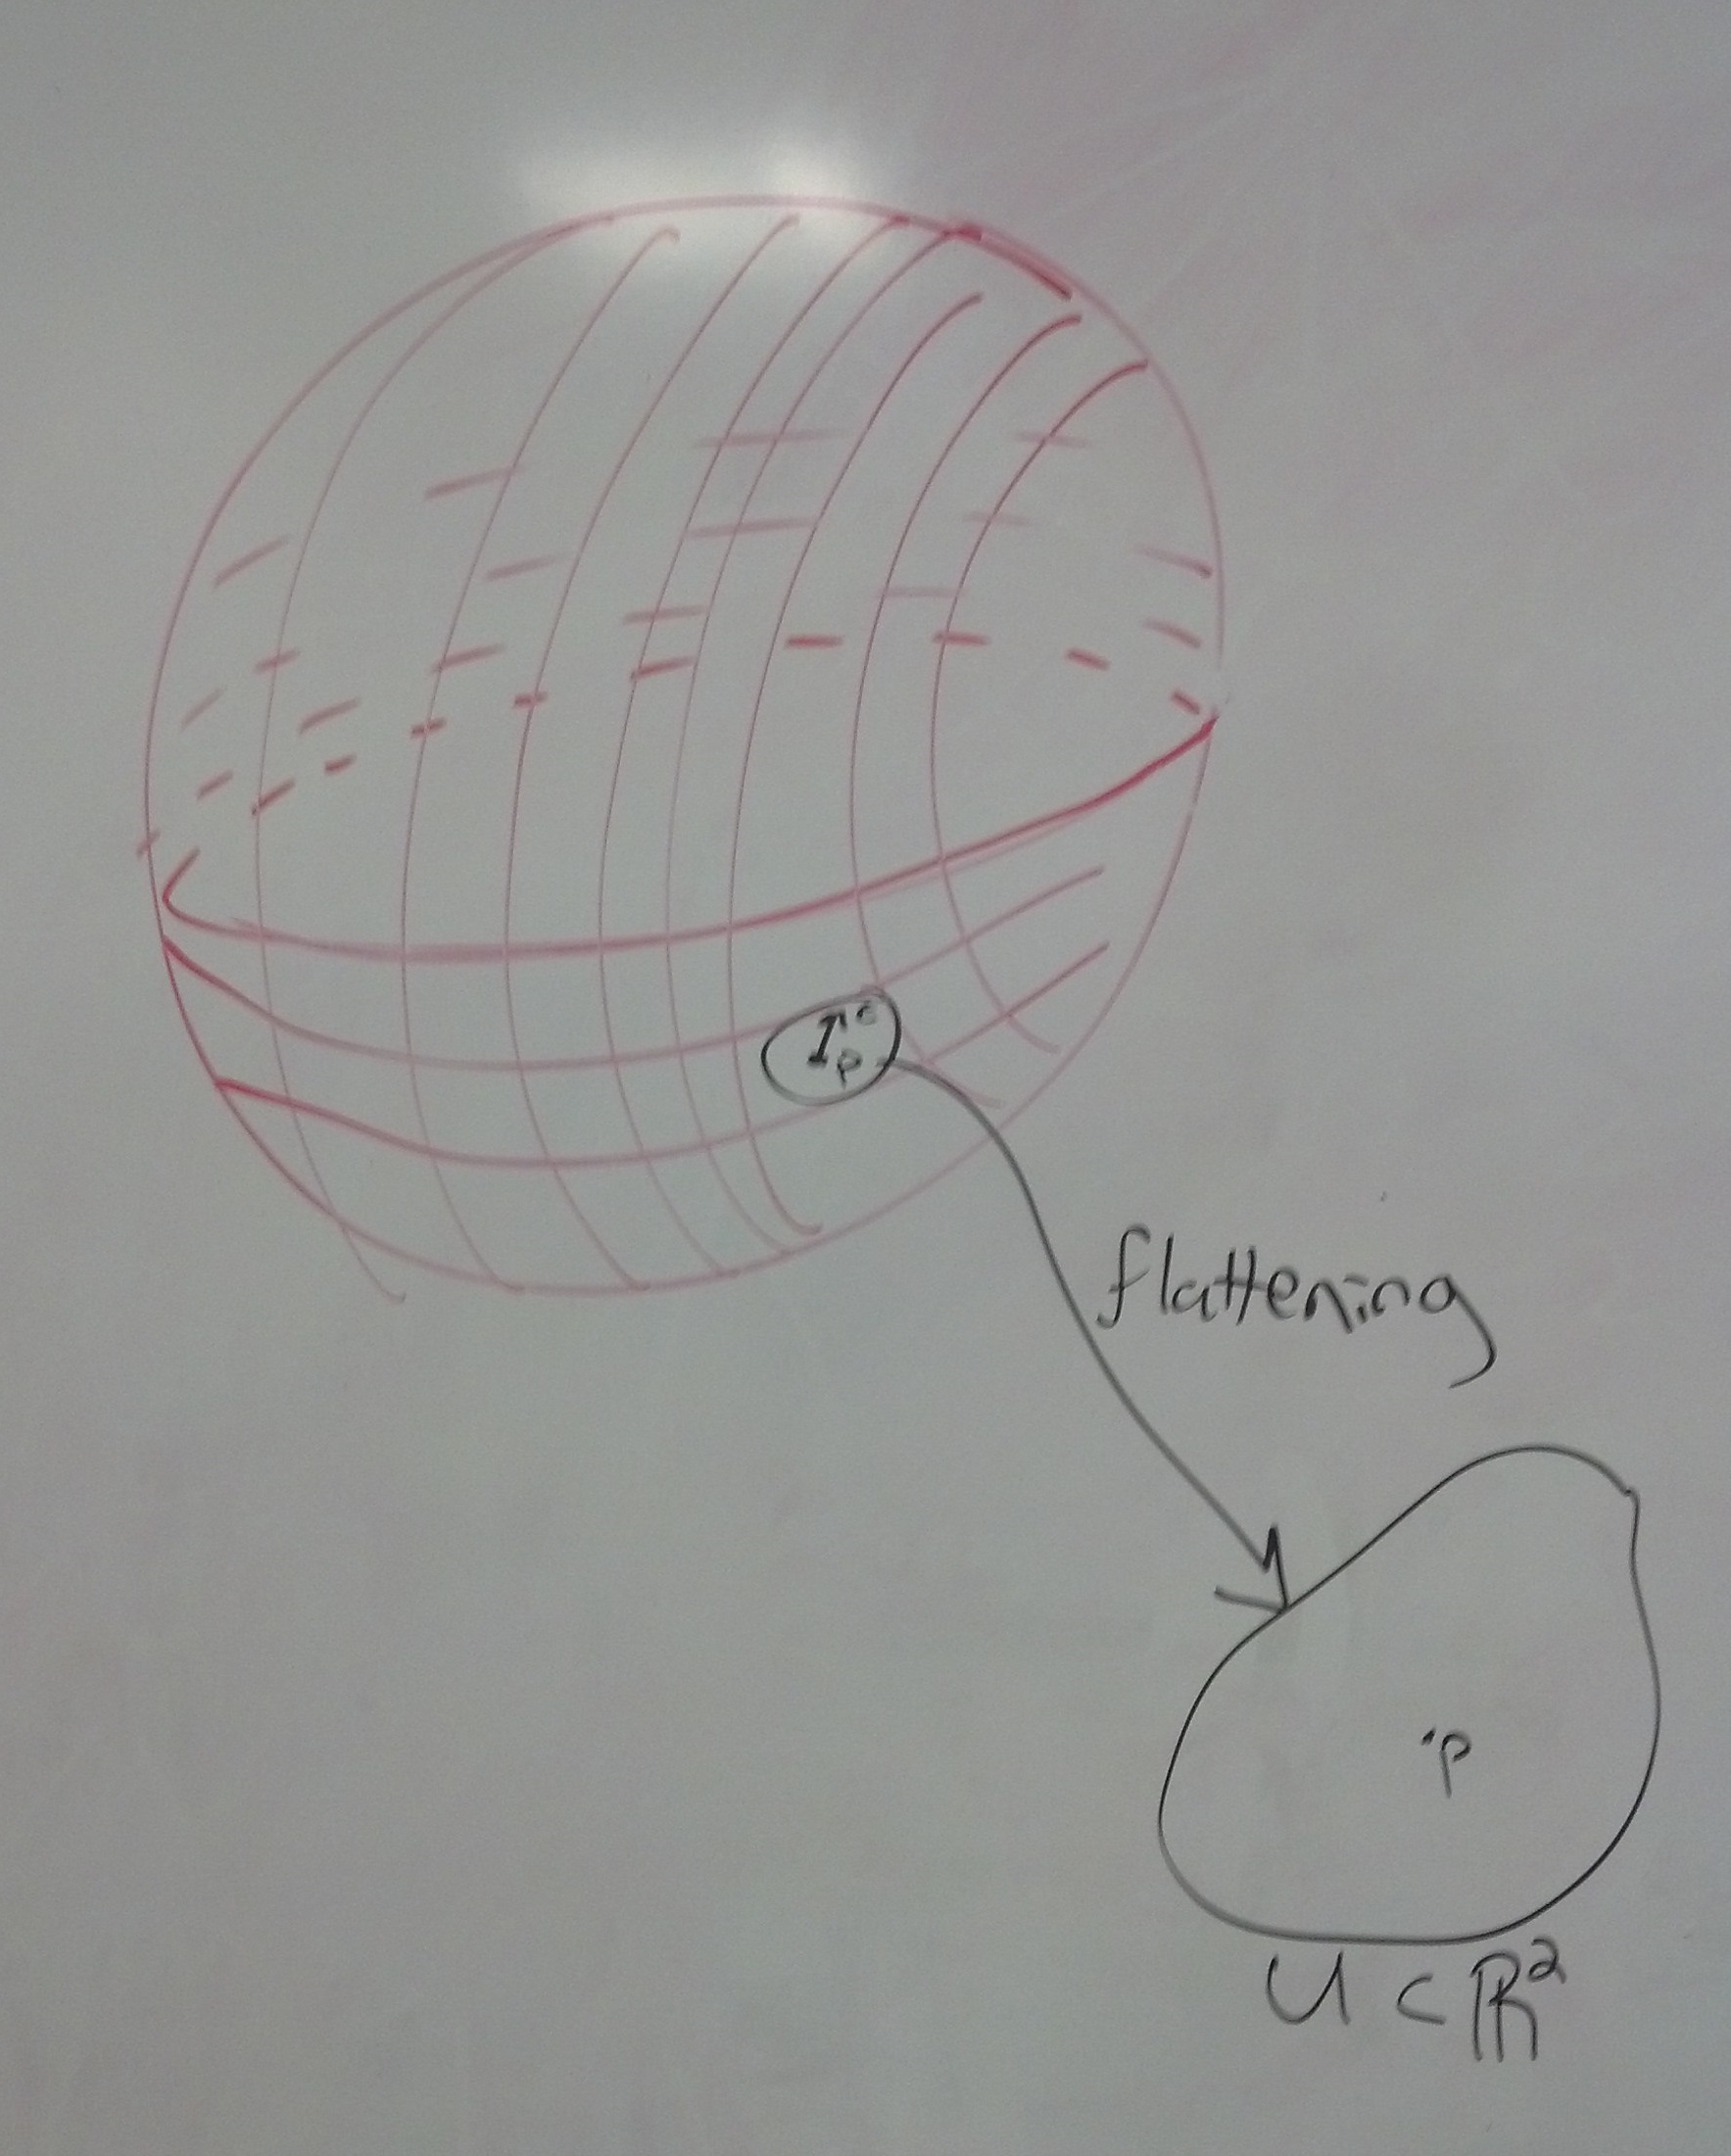
\includegraphics[width=\columnwidth]{manifolddiagram.jpg}
\caption{The manifold with its $\epsilon$ neighborhood at a point $p$}
\label{manifolddiagram}
\end{figure}
